% Generated by code/needham.py -- do not edit by hand.
\definecolor{qocA}{rgb}{0.00,0.45,0.70}
\definecolor{qocB}{rgb}{0.90,0.60,0.00}
\definecolor{qocC}{rgb}{0.00,0.62,0.45}
\definecolor{qocD}{rgb}{0.80,0.40,0.00}
\definecolor{qocE}{rgb}{0.80,0.60,0.70}
\definecolor{qocF}{rgb}{0.35,0.70,0.90}
\begin{tikzpicture}[ink/.style={line width=0.9pt, ndInk}, faint/.style={line width=0.4pt, ndInk!35}, dashedink/.style={line width=0.5pt, ndInk!55, dash pattern=on 2.5pt off 2pt}, vec/.style={->, >=stealth, line width=1.2pt}, note/.style={font=\footnotesize\itshape, text=ndInk!85, align=center}, pointer/.style={->, >=stealth, line width=0.4pt, ndInk!60, shorten >=2pt, shorten <=1pt}, dot/.style={circle, fill=ndInk, inner sep=0pt, minimum size=3.4pt}, wash/.style={fill=ndSky, fill opacity=0.55}, every node/.style={text=ndInk}]
\definecolor{ndInk}{rgb}{0.13,0.13,0.18}
\definecolor{ndPaper}{rgb}{0.99,0.96,0.88}
\definecolor{ndSky}{rgb}{0.84,0.91,0.98}
\definecolor{ndRose}{rgb}{0.98,0.86,0.84}
\definecolor{ndBlue}{rgb}{0.13,0.36,0.66}
\definecolor{ndRed}{rgb}{0.78,0.20,0.16}
\definecolor{ndGold}{rgb}{0.88,0.62,0.10}
\definecolor{ndGreen}{rgb}{0.18,0.52,0.30}
\fill[ndSky, fill opacity=0.55] (0,0) circle (2.200);
\draw[ink] (0,0) circle (2.200);
\draw[faint, ->, >=stealth] (-2.400,0) -- (2.500,0) node[right, font=\scriptsize, text=ndInk] {$x$};
\draw[faint, ->, >=stealth] (0,-2.400) -- (0,2.500) node[above, font=\scriptsize, text=ndInk] {$z$};
\draw[ndGreen!70, line width=0.6pt] (1.866,-1.166) -- (-1.866,1.166);
\node[font=\small, text=ndGreen, anchor=south] at (-1.922,1.201) {$\vec m$};
\draw[line width=2.4pt, ndGreen!55] (0.605,-0.378) -- (0.898,-0.561);
\node[circle, fill=ndBlue, inner sep=0pt, minimum size=3.0pt] at (0.605,-0.378) {};
\node[circle, fill=ndRed, inner sep=0pt, minimum size=3.0pt] at (0.898,-0.561) {};
\draw[ink, line width=0.9pt] (-0.886,-2.014) -- (0.886,2.014);
\node[dot] at (0.886,2.014) {};
\node[dot, fill=white, draw=ndInk] at (-0.886,-2.014) {};
\node[font=\small, anchor=south west] at (0.916,2.014) {$\vec n$};
\node[note, anchor=north east] at (-0.936,-2.034) {outcome $-1$:\\ guess $\sigma$};
\draw[ndBlue, line width=0.5pt, densely dashed] (1.364,0.836) -- (0.529,1.203);
\draw[ndRed, line width=0.5pt, densely dashed] (0.396,-1.364) -- (-0.439,-0.997);
\draw[line width=2.4pt, ndGold!80] (-0.439,-0.997) -- (0.529,1.203);
\node[circle, fill=ndBlue, inner sep=0pt, minimum size=3.4pt] at (0.529,1.203) {};
\node[circle, fill=ndRed, inner sep=0pt, minimum size=3.4pt] at (-0.439,-0.997) {};
\node[font=\small, text=ndGold!60!ndInk, anchor=east] at (-0.376,-0.556) {$2D$};
\draw[ndInk!70, line width=0.7pt] (0.396,-1.364) -- (1.364,0.836);
\draw[vec, ndBlue] (0,0) -- (1.364,0.836);
\draw[vec, ndRed] (0,0) -- (0.396,-1.364);
\node[font=\small, text=ndBlue, anchor=west] at (1.444,0.836) {$\Bloch_\rho$};
\node[font=\small, text=ndRed, anchor=west] at (0.476,-1.384) {$\Bloch_\sigma$};
\node[note, anchor=west] (best) at (2.950,1.45) {the best axis $\vec n$ is parallel to\\ the chord, with the projector\\ $E=\tfrac12(\Id+\vec n\cdot\vec\sigma)$; the shadows\\ of the states on it are as far\\ apart as the states, $2D$};
\draw[pointer] (best.west) to[bend right=15] (0.824,1.873);
\node[note, anchor=west] at (2.950,0.0) {guess $\rho$ on outcome $+1$:\\ right with probability\\ $\tfrac12(1+D)=0.77$};
\node[note, anchor=west, text=ndGreen!80!ndInk] (worse) at (2.950,-1.45) {any other axis $\vec m$ casts\\ closer shadows, and tells\\ the states apart less well};
\draw[pointer] (worse.west) to[bend left=12] (1.642,-1.026);
\end{tikzpicture}
